\speciestitle{Hydroxyl Radical}{OH}{OH}{%
ite\item[Useful range:] 32\,--\,0.0032\,hPa
\item[Contact:] Luis Millan, \email{Luis.F.Millan@jpl.nasa.gov}
  and Shuhui Wang, \email{shw@gps.caltech.edu}}

\subsection{Introduction}

The MLS THz radiometer is dedicated to measuring OH in the 2.5\,THz
spectral region. A description of OH data quality, precision and
systematic errors for an earlier version, v2.2, is given in
\citet{PickettEtal:2006:Validation}. The validation studies are described in
\citet{PickettEtal:2008} and \citet{WangEtal:2008}. While the OH data quality
is generally similar between v2.2 and \prevv, there are significant
improvements in the current version \thisv. In previous versions, OH
data near the mesospheric density peak, \texttildelow0.032 hPa, often
show considerable amount of data flagged with negative precision,
indicating strong influence of \emph{a priori} information, particularly
in the summer hemisphere (or tropics when near the equinox) and
sometimes causes gaps in zonal mean time series. The \thisv software
resolves this issue by fixing the overly tight \texttt{a priori}
constraints. The resulting mesospheric OH data are less noisy and
generally have somewhat larger values than previous versions for the
problematic seasons/latitudes. Another improvement is the smaller bias
at 10\,--\,15\,hPa. Therefore, the day-night correction for bias is only
required for pressure levels at 21 and 32\,hPa. Note that users may
notice more zig-zags in \thisv nighttime mesospheric OH vertical
profiles. This is a side effect of fixing the possible positive bias
introduced by tight lower limits set in previous version retrievals.

The estimated uncertainties, precisions, and resolution for \thisv OH are
summarized in Table~\ref{tab:OHSummary}.

\subsection{Resolution}

Figure~\ref{fig:AvkOH} shows the OH averaging kernel for daytime and
nighttime at 35\degsym N. The reason to separate daytime and nighttime
is that the largest natural variability in OH is diurnal. The vertical
resolution is slightly different between day and night. The nighttime
resolution is sufficient to allow the study of (for example) the
``nighttime OH layer'' around 82\,km.  The vertical width of the
averaging kernel for pressures greater than 0.01\,hPa is\,2.5 km.  The
horizontal width of the averaging kernel is equivalent to a width of
1.5\degsym (165\,km distance) along the orbit.  The changes in vertical
resolution above 0.01\,hPa are due mainly to use of a faster instrument
vertical scan rate for tangent heights above 70\,km.  The horizontal
resolution across track is 2.5\,km. The averaging kernel and resolution
for high and low latitudes are very similar to Figure~\ref{fig:AvkOH}
for most pressure levels.  At the topmost two pressure levels,
0.0046\,hPa and 0.0032\,hPa, the vertical resolution is slightly better
at the equator than at 70\degsym N.

\subsection{Precision}

A typical OH profile and the associated precisions (for both \prevv and
\thisv) are shown in Figure~\ref{fig:OHprofiles}. The profile is shown in
both volume mixing ratio (vmr) and density units. All MLS data are
reported in vmr for consistency with the other retrieved molecules.
However, use of density units (10\cp{6}\,cm\cp{$-$3}) reduces the
apparent steep gradient of OH vertical profile, allowing one to see the
profile with more detail, especially in the stratosphere where most
atmospheric OH is present.  Additionally, at THz frequencies the
collisional line-width is approximately equal to the Doppler width at
1\,hPa. Above 1\,hPa, Doppler broadening is dominant and the peak
intensity of OH spectral absorption is proportional to density, while
below 1\,hPa the peak intensity is proportional to vmr. The daytime OH
density profile shows two peaks at \texttildelow45\,km and \texttildelow75\,km. The
night OH profile exhibits the narrow layer at \texttildelow82 km
\citep{PickettEtal:2006:NightOH}. Precisions are such that an OH zonal
average within a 10\degsym\ latitude bin can be determined with better
than 10\% relative precision with one day of data (\texttildelow100 samples)
over 21\,--\,0.01\,hPa. With 4 days of data, the 10\% precision limits
can be extended to 32\,--\,0.0046\,hPa.

\begin{figure}
\centering\includegraphics[width=0.7\linewidth]{figures/avk-OH}
  \caption{Typical two-dimensional (vertical and horizontal along-track)
    averaging kernels for the MLS \thisv OH data at 35\degsym N for
    daytime (upper) and nighttime (lower); variation in the averaging
    kernels is sufficiently small that these are representative of
    typical profiles. Colored lines show the averaging kernels as a
    function of MLS retrieval level, indicating the region of the
    atmosphere from which information is contributing to the
    measurements on the individual retrieval surfaces, which are denoted
    by plus signs in corresponding colors. The dashed black line
    indicates the resolution, determined from the full width at half
    maximum (FWHM) of the averaging kernels, approximately scaled into
    kilometers (top axes). (Left) Vertical averaging kernels (integrated
    in the horizontal dimension for five along-track profiles) and
    resolution.  The solid black line shows the integrated area under
    each kernel (horizontally and vertically); values near unity imply
    that the majority of information for that MLS data point has come
    from the measurements, whereas lower values imply substantial
    contributions from a priori information. (Right) Horizontal
    averaging kernels (integrated in the vertical dimension) and
    resolution.  The averaging kernels are scaled such that a unit
    change is equivalent to one decade in pressure.}
\label{fig:AvkOH}
\end{figure}

\begin{figure}
\begin{tabular}{@{}l@{}l@{}}
\includegraphics[width=0.5\linewidth]{figures/plot-OHv4-a}&
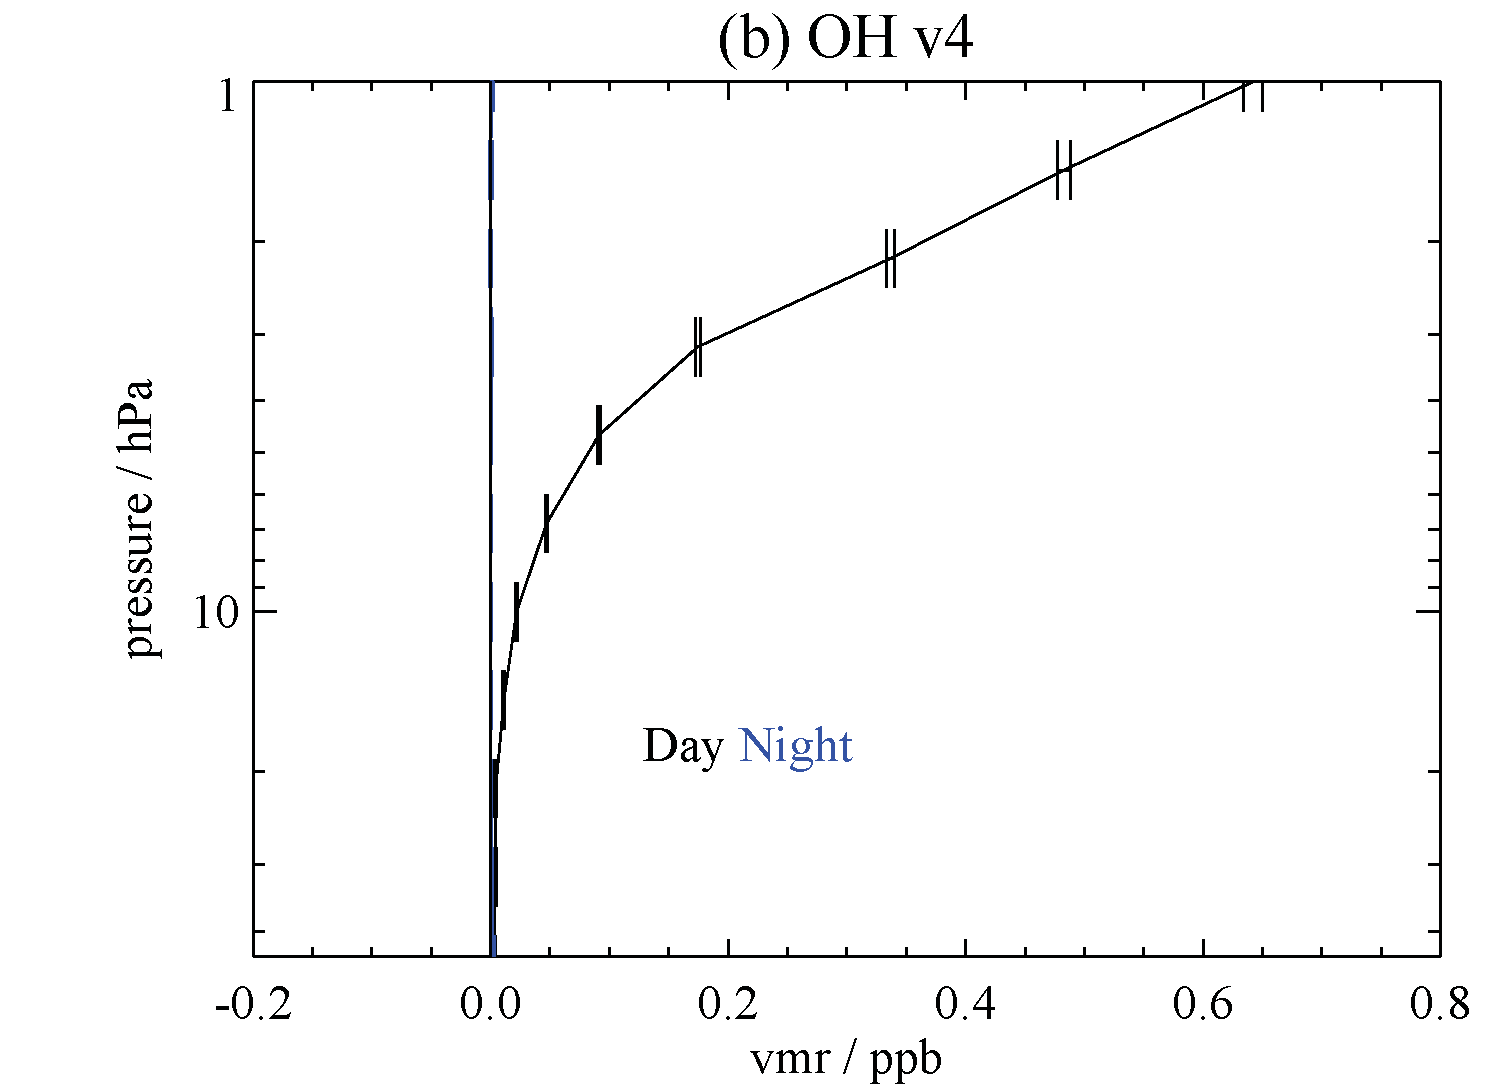
\includegraphics[width=0.5\linewidth]{figures/plot-OHv4-b}\\
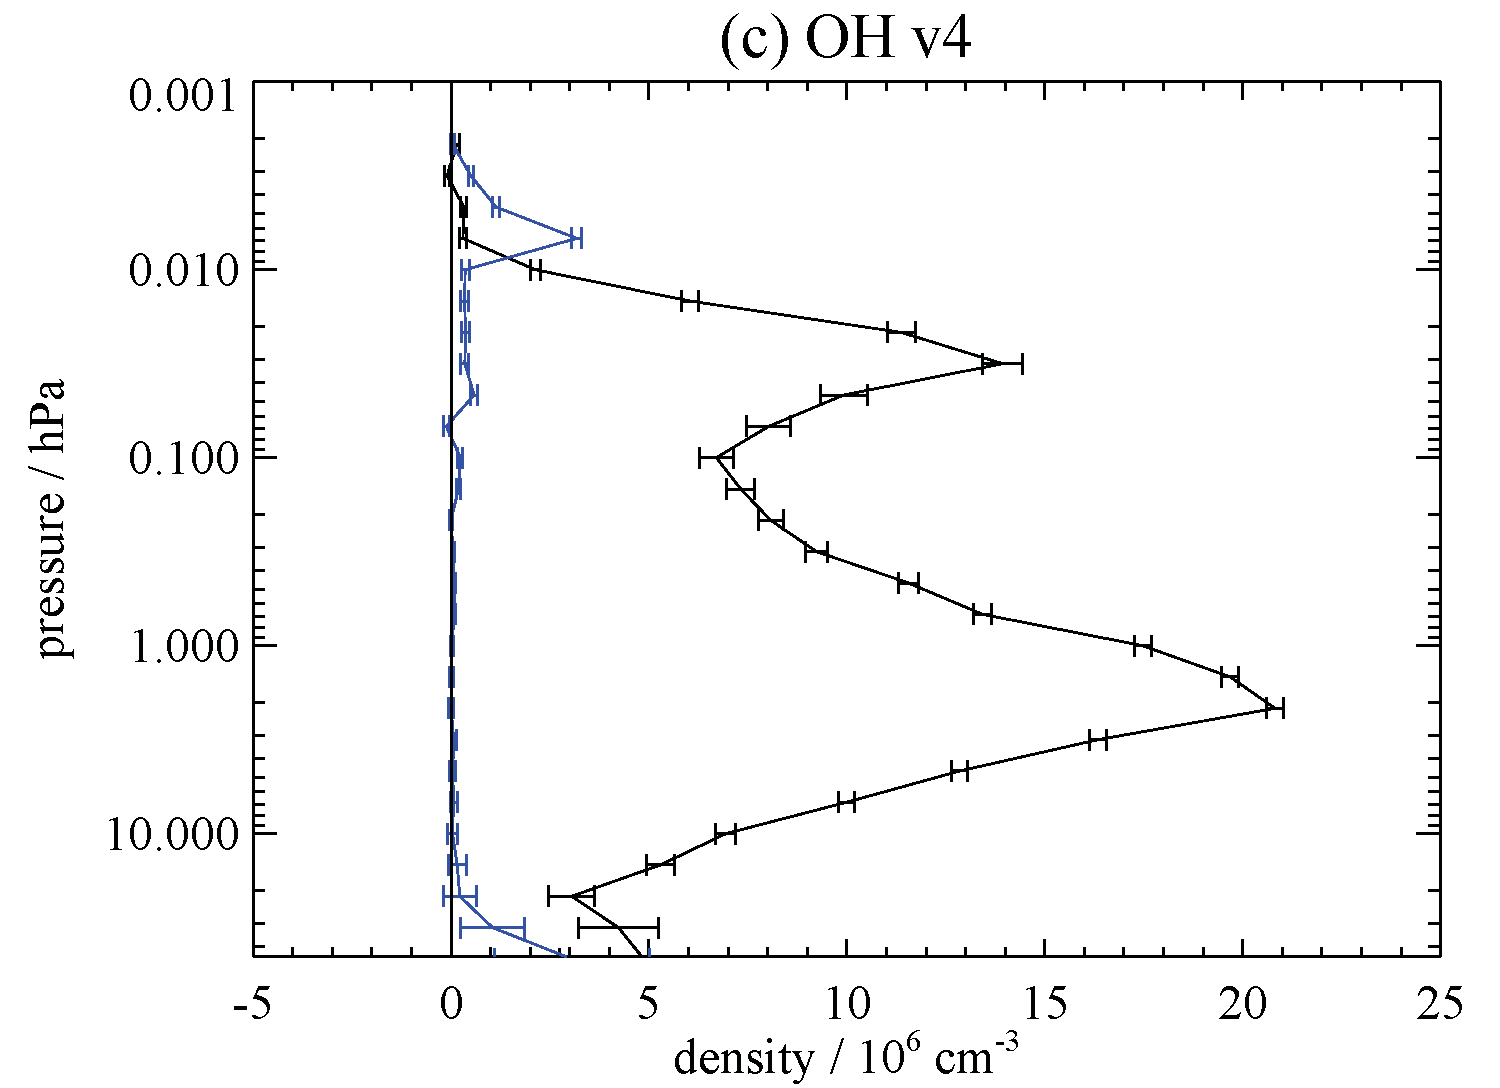
\includegraphics[width=0.5\linewidth]{figures/plot-OHv4-c}&
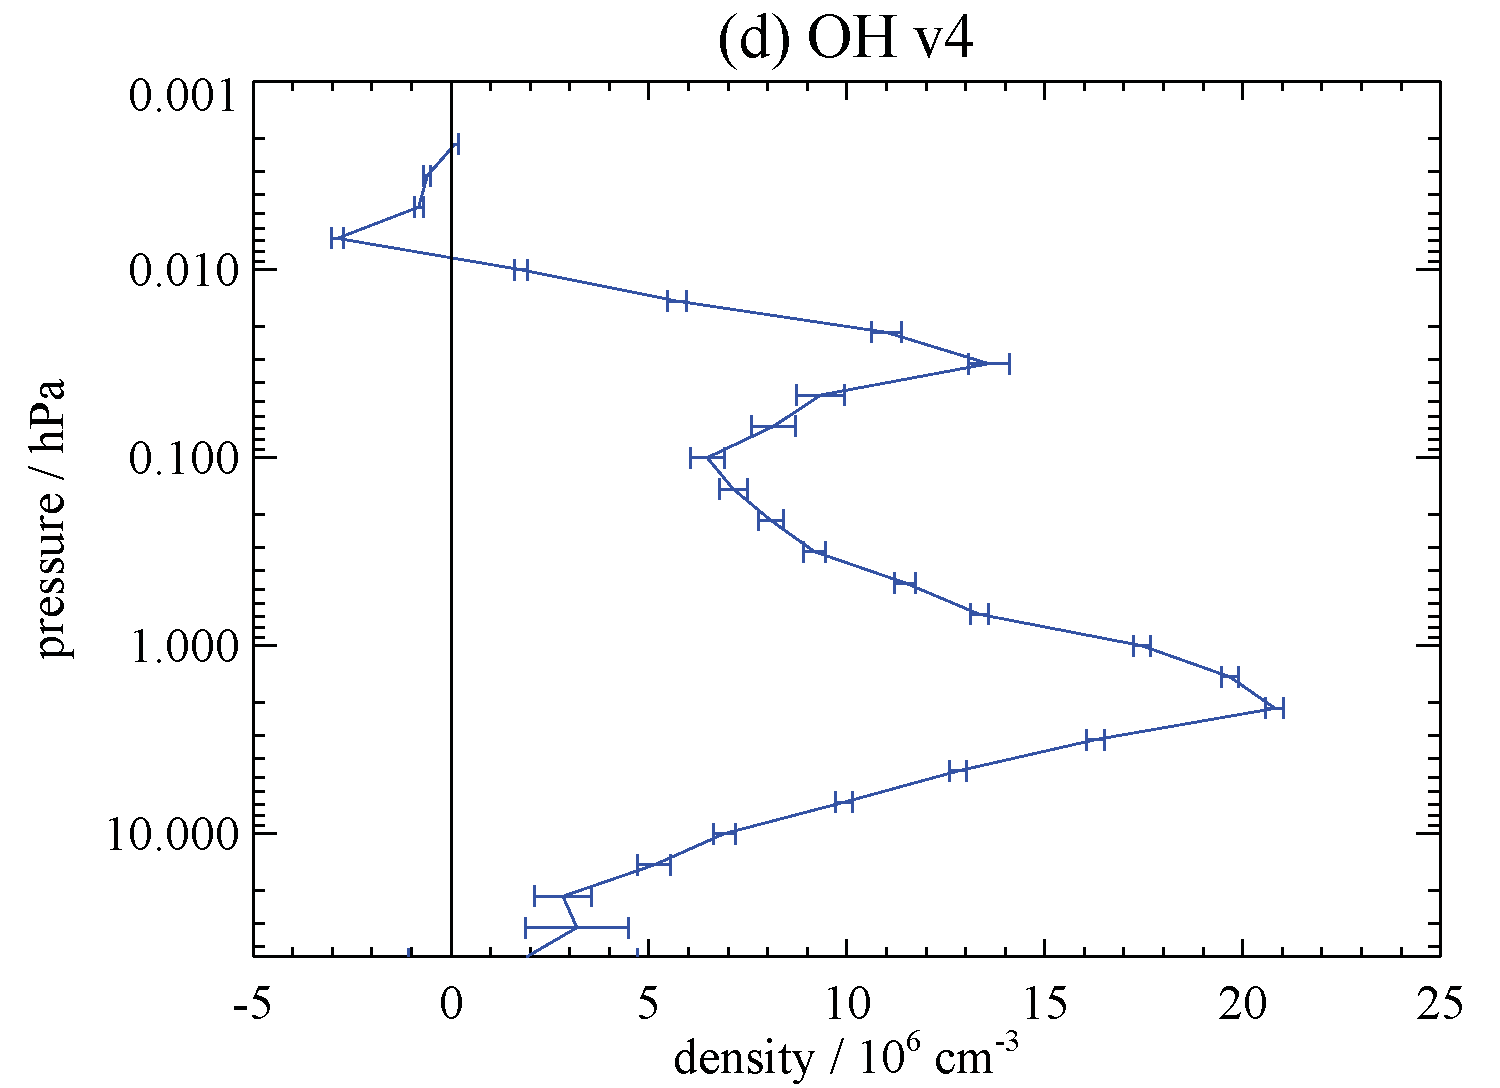
\includegraphics[width=0.5\linewidth]{figures/plot-OHv4-d}\\
\includegraphics[width=0.5\linewidth]{figures/plot-OHv3-e}&
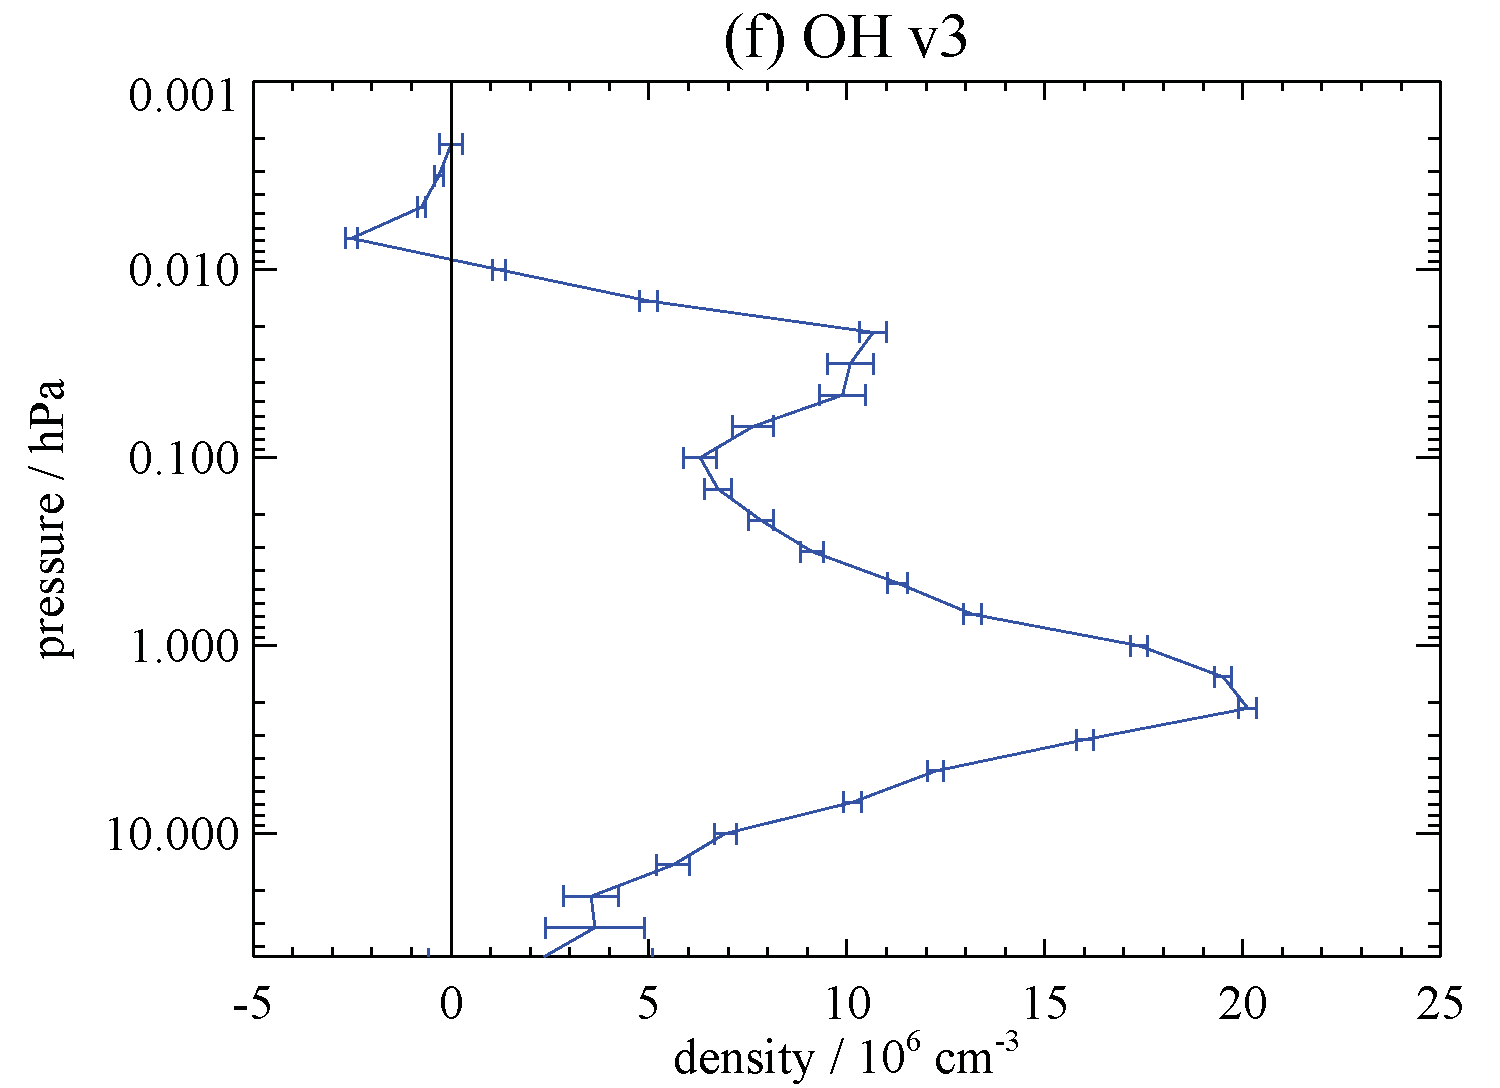
\includegraphics[width=0.5\linewidth]{figures/plot-OHv3-f}%
\end{tabular}
\caption{Zonal mean of retrieved OH and its estimated precision
  (horizontal error bars) for September 20, 2005 averaged over 29\degsym
  N to 39\degsym N\@. The average includes 98 profiles. Panel (a) shows
  \thisv OH vmr vs. pressure for day (black) and night (blue).  Panel (b)
  shows the same data plotted for the stratosphere. The retrieved night
  OH concentration is near zero for altitudes below 1\,hPa.  Panel (c)
  shows the same data in (a) converted into density units.  Panel (d)
  shows the day-night differences for the data in panel (c).  Note that
  the day-night difference is required for altitudes below 20\,hPa.
  Panels (e) and (f) are equivalent to (c) and (d) but using \prevv OH
  data.}
\label{fig:OHprofiles}
\end{figure}


\subsection{Accuracy}

Table~\ref{tab:OHSummary} summarizes the accuracy expected for OH\@.
The effect of each identified source of systematic error on MLS
measurements of radiance has been quantified and modeled
\citep{ReadEtal:2007}. These quantified effects correspond to either
$2\sigma$ estimates of uncertainties in each MLS product, or an estimate
of the maximum reasonable uncertainty based on instrument knowledge
and/or design requirements.These accuracy calculations were performed
with more realistic OH atmospheric profiles than for \prevv
estimates. Biases can be eliminated by taking day-night differences from
32\,--\,21\,hPa. For 15\,--\,0.1\,hPa, the observed night OH
concentration is small and day-night differencing is not ordinarily
needed. The overall uncertainty is the square root of the sum of squares
of the precision and accuracy.

\subsection{Data screening}
\label{sec:OHScreening}
It is recommended that OH data values be used in scientific
investigations if all the following tests are successful:

\begin{description}
\item[Pressure range:] \screeningrule{32\,--\,0.0032\,hPa.}
  \standardrangestatement
\standardprecisionrule
\evenstatusrule
\item[Quality:] \screeningrule{MLS \thisv OH data can be used
    irrespective of the value of the \texttt{Quality} field.}
\item[Convergence:] \convergencerule{1.1}
\end{description}

\subsection{Artifacts}

For some seasons, the Gas Laser Local Oscillator (GLLO) for the THz
receiver is automatically ``relocked'' as many as 5 times during a day,
leading to data gaps.  In these cases the \texttt{Status} flag is set to
\texttt{257} and the profile is ignored. This can present a problem when
compiling maps, because the missing data may appear at the same latitude
and longitude on successive days.

\subsection{Review of comparisons with other datasets}

Data from MLS v2.2 software have been validated with two balloon-borne
remote-sensing instruments and with ground-based column measurements.
Details of the comparison are given in \citet{PickettEtal:2008} and
\citet{WangEtal:2008}.  The comparison among v2.2, \prevv, and \thisv show
no significant differences except for the mesosphere where \thisv OH
daytime values are somewhat larger and less noisy in the summer
hemisphere (or tropics when near equinox).

\begin{table}
\caption{Summary of precisions, resolution, and uncertainties for the
  MLS OH product}
\vspace{\tablecaptionsep}
\label{tab:OHSummary}
\begin{minipage}{\textwidth}\small
\centering\begin{tabular}{rcccl}
\toprule
\textbf{Pressure} &
\parbox{6em}{\bfseries\centering Resolution\\ V $\times$ H /km} &
\parbox{5em}{\bfseries\centering Precision\footnote{Precision on an
    individual profile} (day/night) / 10\cp6 cm\cp{$-$3}} &
\parbox{5em}{\bfseries\centering Accuracy / 10\cp6 cm\cp{$-$3}} &
\textbf{Comments}\\
\midrule
$<$0.003\,hPa     & ---                  & ---                  & ---   &  Unsuitable for scientific use\\
0.003\,hPa        & 5.0 $\times$ 220     & 0.5 / 0.5            & 0.5 & \\
0.01 \,hPa        & 2.5 $\times$ 180     & 1.1 /1.1             & 2   & \\
0.1\,hPa          & 2.5 $\times$ 165     & 3.3 / 0.6            & 1.0  & \\
1.0\,hPa          & 2.5 $\times$ 165     & 1.9 / 0.4            & 1.0  & \\
10 \,hPa          & 2.5 $\times$ 165     & 2.3 / 1.4            & 0.9  & \\
32\,--\,14\,hPa   & 2.5 $\times$ 165     & 6\,--\,10 / 4\,--\,8 & 1.3  & Use day--night difference \\
$>$32\,hPa        & ---                  & ---                  & ---   & Unsuitable for scientific use\\
\bottomrule
\end{tabular}
\end{minipage}
\end{table}

%%% Local Variables:
%%% mode: latex
%%% TeX-master: "v5-x-report"
%%% End:
